\begin{lem}
    \label{lem:manifolds_1}
    For any collection of \(n - m + 1\) vertices \(\{v_\alpha\}_{\alpha=m}^n\)
    in \(\Gamma - \{v_\alpha,  w_\alpha\}_{\alpha=1}^{m-1}\), there exists exactly two edges
    \(e_1 = v_i u_1\) and \(e_2 = v_j u_2\) such that
    \begin{enumerate}[label=(\roman*)]
    \item \(m \leq i, j \leq n\)
    \item \(u_1, u_2 \not \in \{v_\alpha\}_{\alpha=1}^n\cup\{w_\alpha\}_{\alpha=1}^{m-1}\)
    \item Exactly one of the following hold in Figure \ref{fig:lem:manifolds_1}
    \end{enumerate}
    \begin{figure}[h!]
        \centering
        \begin{enumerate*}[label=(\arabic*)]
            \item \label{fig:lem:manifolds_1_1}
            \begin{minipage}{.3\textwidth}
                \centering
                \(v_i = v_j\) \textit{and} \(u_1 \neq u_2\) \\
                \vspace{1em}
                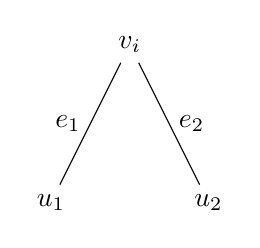
\begin{tikzpicture}
                    \node (vi) at (3, 2) {\(v_i\)};
                    \node (w2) at (2, 0) {\(u_1\)};
                    \node (w3) at (4, 0) {\(u_2\)};

                    \draw (vi) -- (w2) node[midway, left] {\(e_1\)};
                    \draw (vi) -- (w3) node[midway, right] {\(e_2\)};
                \end{tikzpicture} 
            \end{minipage}

            \hspace{3em}

            \item \label{fig:lem:manifolds_1_2}
            \begin{minipage}{.3\textwidth}
                \centering
                \(u_1 = u_2\) \textit{and} \(v_i \neq v_j\) \\
                \vspace{1em}
                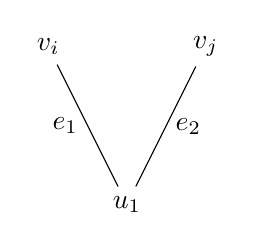
\begin{tikzpicture}
                    \node (vi) at (2, 2) {\(v_i\)};
                    \node (vj) at (4, 2) {\(v_j\)};
                    \node (w2) at (3, 0) {\(u_1\)};

                    \draw (vi) -- (w2) node[midway, left] {\(e_1\)};
                    \draw (vj) -- (w2) node[midway, right] {\(e_2\)};
                \end{tikzpicture}
            \end{minipage}
        \end{enumerate*}
        \caption{Lemma \ref{lem:manifolds_1} possibilities.}
        \label{fig:lem:manifolds_1}
    \end{figure}
\end{lem}

\begin{proof}
    Let \(\{v_\alpha\}_{\alpha=m}^n\) be a collection of \(n - m + 1\) vertices in \(\Gamma - \{v_\alpha, w_\alpha\}_{\alpha=1}^{m-1}\)
    and put a particle at each vertex in \(\{v_\alpha\}_{\alpha=1}^n\).
    The movements of the particles from \((v_\alpha)_{\alpha=1}^{m-1}\) to \((w_\alpha)_{\alpha=1}^{m-1}\)
    correspond to an \((m-1)\)-cube in \(\DConf_n(\Gamma)\).
    Since the configuration space is an \(m\)-manifold without boundary, 
    this \((m-1)\)-cube must border exactly two distinct \(m\)-cubes.
    For this \((m-1)\)-cube to border two \(m\)-cubes,
    there needs to exist two additional mutually exclusive particle movements.
    Let \(v_i, v_j \in \{v_\alpha\}_{\alpha=m}^n\) be the vertices that these particles occupy.
    Since the particle(s) at \(v_i\) and \(v_j\) need to move simultaneously as the particles move from \((v_\alpha)_{\alpha=1}^{m-1}\) to \((w_\alpha)_{\alpha=1}^{m-1}\),
    there exist destination(s) \(u_1\) and \(u_2\) outside the set \(\{v_{\alpha}\}_{\alpha=1}^n \cup \{w_\alpha\}_{\alpha=1}^{m-1}\).
    In order for these additional movements to be mutually exclusive, either \(v_i \neq v_j\) or \(u_1 \neq u_2\) but not both.
\end{proof}


\begin{lem}
    Suppose \(\DConf_n(\Gamma)\) is an \(m\)-manifold without boundary and let \(M\) be an \(m-1\) matching in \(\Gamma\).
    For any vertex \(v\) in \(\DConf_{n - (m - 1)}(\Gamma - N(M))\), there exists exactly two distinct edges incident to \(v\).
\end{lem}

\begin{proof}
Let \(v\) be a vertex in \(\DConf_{n - (m - 1)}(\Gamma - N(M))\).
Consider the configuration of \(n\) particles placed such that \(m-1\) are placed on the edges in \(M\)
and the remaining \(n - (m-1)\) particles are placed on each component of \(v\).

As the particles on the edges in \(M\) move, an \((m-1)\)-cube is spanned in \(\DConf_n(\Gamma)\).
Since \(\DConf_n(\Gamma)\) is an \(m\)-manifold without boundary,
this \((m-1)\)-cube must border exactly two distinct \(m\)-cubes.
For this to happen, there need to be exactly two additional mutually exclusive particle movements.
There are only two ways for this to happen:
\begin{enumerate}
    \item Only a single particle is able to travel to two distinct vertices in \(\Gamma - N(M)\).
    \item Two distinct particles are each able to travel to a common vertex in \(\Gamma - N(M)\).
\end{enumerate}
In either case, these movements correspond to two distinct edges incident to the vertex \(v\) in \(\DConf_{n - (m - 1)}(\Gamma - N(M))\).

\end{proof}

\begin{lem}
    Suppose \(\DConf_n(\Gamma)\) is an \(m\)-manifold without boundary and let \(M\) be an \((m-1)\)-matching in \(\Gamma\).
    Then, \(\DConf_{n - (m - 1)}(\Gamma - N(M))\) is a \(1\)-manifold without boundary.
\end{lem}

\begin{proof}
    By the previous lemma, every vertex in \(\DConf_{n - (m - 1)}(\Gamma - N(M))\) has exactly two incident edges.
    Therefore, \(\DConf_{n - (m - 1)}(\Gamma - N(M))\) is one or more disjoint cycles.
\end{proof}


\begin{thm}
    Suppose \(\DConf_n(\Gamma)\) is an \(m\)-manifold without boundary and let \(M\) be a \((m-k)\)-matching in \(\Gamma\).
    Then, \(\DConf_{n - (m-k)}(\Gamma - N(M))\) is a \(k\)-manifold without boundary.
\end{thm}

\begin{proof}
    We proceed by induction on \(k\). The base case \(k = 1\) was shown in the previous lemma.
    So, suppose the result holds for some \(k \ge 1\) and let \(M\) be an \((m - k - 1)\)-matching in \(\Gamma\).

    Let \(v\) be a vertex in \(\DConf_{n - m + k + 1}(\Gamma - N(M))\).
    Let \(p\) be a configuration of \(n\) particle placed on \(\Gamma\) 
    such that \(m - k - 1\) are on \(M\) and \(n - m + k + 1\) are placed at \(v\).
    As the particles on \(M\) move, an \(m - k - 1\) cube \(C\) is spanned in \(\DConf_n(\Gamma)\).
    Since \(\DConf_n(\Gamma)\) is an \(m\)-manifold, \(C\) cube must belong
    to \(2^{m - (m - k -1)} = 2^{k+1}\) distinct \(m\)-cubes in \(\DConf_n(\Gamma)\).

    Each \(m\)-cube that \(C\) belongs to contains \(p\).
    An \(m\)-cube is spanned in \(\DConf_n(\Gamma)\) only when \(m\) distinct particles move simultaneously.
    Since the particles on \(M\) already are moving to span \(C\), 
    % FALSE 2^{m - k} no work maybe this is recoverable when there are just at least 2 additional.
    % idk this approach going on the backburner
    there are \(2^{k+1}\) mutually exclusive ways for all \(n - m + k + 1\) particles at \(v\) to move simultaneously.
    Each of these \(2^{k+1}\) ways for particles to move at \(v\) corresponds to an edge incident to \(v\) in
    \(\DConf_{n - w + k + 1}(\Gamma - N(M))\).
    Let \(w\) be a vertex in \(\DConf_{n - w + k + 1}(\Gamma - N(M))\) distinct from \(v\) but incident to
    one of these edges.
    
    
\end{proof}
